%Building
\documentclass[11pt]{article}

\usepackage[english]{babel}
\usepackage[margin=1in]{geometry}
\usepackage[colorlinks=true, allcolors=blue]{hyperref}

% Math/Greek packages
\usepackage{amssymb, amsmath, amsthm, mathtools, esint} 
\usepackage{algorithm, algorithmic}
\usepackage{upgreek}
\usepackage{physics}

% Graphics/Presentation packages
\usepackage{graphicx}
\usepackage{multirow, subcaption, cleveref}
\usepackage{tabulary, enumitem}
\usepackage{cancel}

%replace "ref" with "cref", "Cref", "crefrange"

% Misc packages
\renewcommand\qedsymbol{\textit{``Quack"}} %change the QED symbol to ``Quack" for the inside joke of Quantum Entangled Ducks

% defining where the images are
\graphicspath{ {../ESOF 322 Project (drive copy)/} }



\begin{document}

\title{ESOF 322: Project 1 - Cold Case Database}
\author{Jacob Coleman, William Jardee, Fletcher Philips, Megan Steinmasel}
\maketitle


%%TO-DO
% check for any implementation in usecases

\textbf{System Description}: In the world of criminal justice, it is not a rare occurrence that the truth is thinly veiled by a lack of gathered evidence or proper techniques to analyze current data. A prime example of this is the aid of DNA testing in prosecution. The proposed software system will collect old and new evidence into one database, organize it, and present it to domain specialists through an easy-to-use website. The initial construction of this project is humble but aims to create a skeleton for more sophisticated analysis techniques to be built on. It is assumed that there are two primary ways to interact with the system: through back-end control of the database operations and layman's interpretation of the data in the form of a website; these are the database engineer and website user, respectively. Throughout this whole document, it is assumed that the web servers and hardware maintenance are outside the scope of the software; however, it would make logical sense for the same database engineer to be educated on that system and in charge of it completely as there will likely be an error that occurs between the two systems. \vspace{1.5em}

\textit{Database Engineer}: An individual knowledgeable of how the system works and responsible for maintenance and updates.\vspace{0.5em}

\textit{Website  User}: A front-end user that likely lacks data science knowledge traversing the web system.\vspace{1.5em}


\section*{User Stories}

\noindent\textbf{Epic}: As a criminal justice professional, I want a general database that can hold, sort, and present data according to a variety of different queries and eventually use state-of-the-art algorithms to help me succeed in my job.\vspace{0.5em}

\noindent\textbf{\hypertarget{us1}{User Story 1}} (Megan Steinmasel):  As a website user, I want a functional web interface that includes a navigation menu and search bar so that I can access information easily.\vspace{0.5em}

\noindent\textbf{\hypertarget{us2}{User Story 2}} (William Jardee): As a website user, I need the processing of new data to find important features and calculate relevant statistics to be done automatically, so it is friendly to someone that is not a data scientist.\vspace{0.5em}

\noindent\textbf{\hypertarget{us3}{User Story 3}} (Jacob Coleman): As a website user, I want a data visualization technique that is intuitive and accurately shows patterns in the data.\vspace{0.5em}

\noindent\textbf{\hypertarget{us4}{User Story 4}} (Fletcher Philips): As a database engineer, I want to have a database so that I can store cold cases inside of it. \vspace{0.5em}

\noindent\textbf{\hypertarget{us5}{User Story 5}} (Fletcher Philips): As a database engineer, I want the data to be manipulable so that the admin can insert and delete data from the database.\vspace{0.5em}

\clearpage
%-----------------------------------------------------------------------------------------
%-----------------------------------------------------------------------------------------



\section{UseCase Diagram}

\begin{figure}[!ht]
\centering
\textbf{Author: William Jardee}
	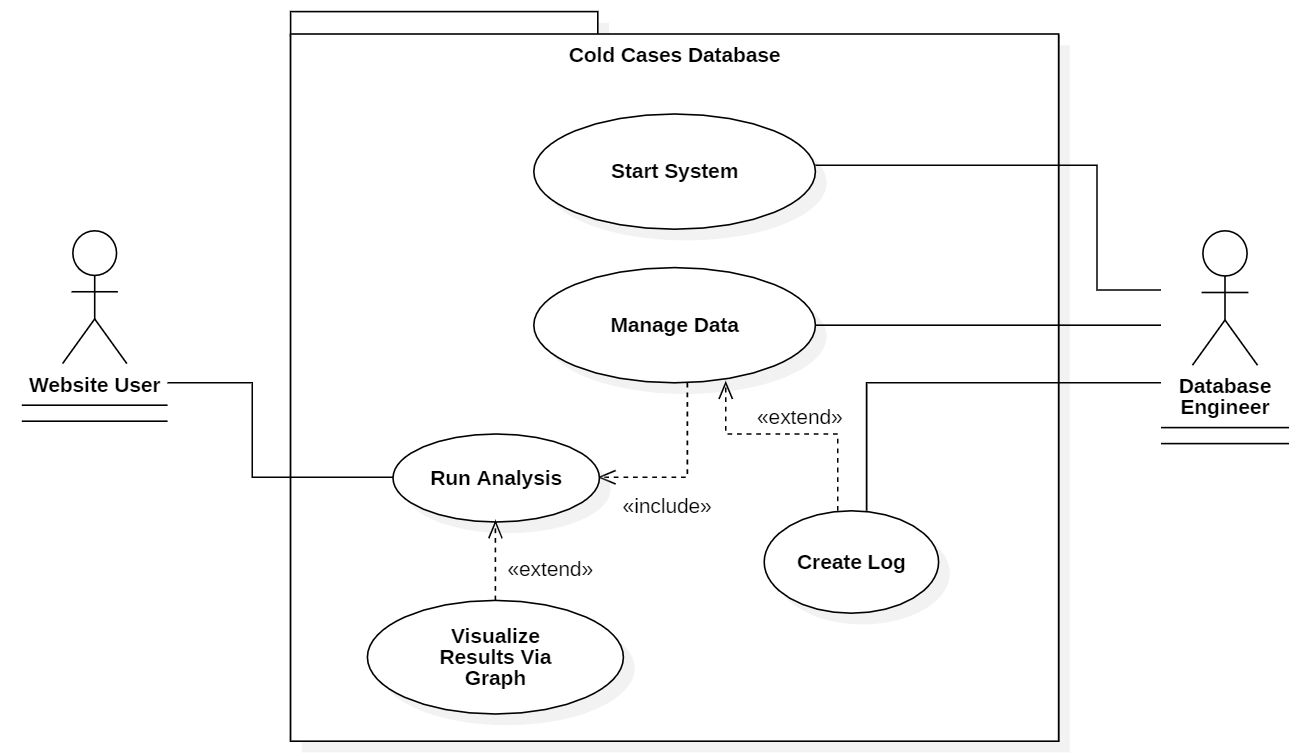
\includegraphics[width=.95\textwidth]{./UseCases/jardee_usecase}\\
	\caption{UseCase Diagram for the Cold-Cases Database system.}
	\label{fig:usecase_diagram}
\end{figure}
\clearpage



\subsection{Textual Descriptions}

%------------------------------------
%Create Database
%------------------------------------
\begin{table}[!ht]
\begin{center}
\textbf{Author: Fletcher Philips}
\vspace*{1em}

\begin{tabular}{p{0.30\linewidth}p{0.60\linewidth}}
	Name: & Create Database/Start System\\\hline
	Description: & A database needs to be created and connected to the web framework we choose.\\\hline
	Related Requirements:& \hyperlink{us4}{User Story 4}\\\hline
	Preconditions:& Basic web infrastructure has been created. A small sample set of cold cases is ready to be inserted.\\\hline
	Successful end condition:& Basic database has been initialized with a substructure. Data has been inserted into the database.\\\hline
	Failed end condition:& Data cannot be inserted into the database.\\\hline
	Actors:& Database Engineer\\\hline
	Basic Flow of Events: & \begin{enumerate}
	\item Create Database.
	\item Connect a database to the web framework.
	\item Insert Initial Data into Database.
	\end{enumerate}\\\hline
	Extensions/Exceptional Flow of Events & \begin{enumerate}
	\item Database fails to build properly.
	\item The engineer is notified that an error has appeared.
	\item Write to log file.
	\item Engineer is ejected from the system.
	\end{enumerate}
\end{tabular}
\label{des:create_database}	
\end{center}
\end{table}
%------------------------------------

%------------------------------------
%Manage Data
%------------------------------------
\begin{table}[!ht]
\begin{center}
\textbf{Author: William Jardee}
\vspace*{1em}

\begin{tabular}{p{0.30\linewidth}p{0.60\linewidth}}
	Name: & Manage Data\\\hline
	Description: & Data needs to be inserted, deleted, and manipulated. Related to this, there must be an appropriate Graphical User Interface. The data will connect directly with the database.\\\hline
	Related Requirements:& \hyperlink{us2}{User Story 2}, \hyperlink{us5}{User Story 5}\\\hline
	Preconditions:& The user is logged on and has gained access rights according to their credentials.\\\hline
	Successful end condition:& Data is successfully manipulated, and a success message is received from the source. \\\hline
	Failed end condition:& Requested task is outside of credentials. Success message not received. Invalid new data.\\\hline
	Actors:& Database Engineer\\\hline
	Basic Flow of Events: & \begin{enumerate}
	\item Actor selects the action they wish to commit and what to commit it on.
	\item Action is tested against credentials.
	\item Success/Fail state is determined.
	\item Flow is complete and prompts the user for the next action.
	\end{enumerate}\\\hline
	Extensions/Exceptional Flow of Events & \begin{enumerate}
	\item Conflict happens.
	\item Reject any attempted changes and revert to the last viable state.
	\item Notify the actor that there has been an error and write to the log file.
	\item Flow is complete and prompts the user for the next action.
	\end{enumerate}
\end{tabular}
\label{des:man_dat}	
\end{center}
\end{table}
%------------------------------------


%------------------------------------
%Run Analysis
%------------------------------------
\begin{table}[!ht]
\begin{center}
\textbf{Author: William Jardee}
\vspace*{1em}

\begin{tabular}{p{0.30\linewidth}p{0.60\linewidth}}
	Name: & Run Analysis\\\hline
	Description: & Graphic User Interface for viewing data and selecting data visualization.\\\hline
	Related Requirements:& \hyperlink{us2}{User Story 2}, \hyperlink{us3}{User Story 3}\\\hline
	Preconditions:& The website user has signed into the website and accessed the drop-down menu to access the page. \\\hline
	Successful end condition:& A valid group of data is selected, a visualization format is selected, and the servers are available for the request.\\\hline
	Failed end condition:& One of the above three requirements has been violated, and the window is closed.\\\hline
	Actors:& Website User\\\hline
	Basic Flow of Events: & \begin{enumerate}
	\item A query selection screen is presented, and the desired data is collected.
	\item The type of visualization is selected from a dropdown menu.
	\item The request is sent to the ``Visualize Results via Graph" action.
	\end{enumerate}\\\hline
	Extensions/Exceptional Flow of Events & \begin{enumerate}
	\item One of the system-side error states was reached.
	\item Report the error to the actor.
	\item Write error to log file.
	\item Return actor back to the homepage.
	\end{enumerate}
\end{tabular}
\label{des:run_anal}	
\end{center}
\end{table}
%------------------------------------


%------------------------------------
%Visualize Results via Graphs
%------------------------------------
\begin{table}[!ht]
\begin{center}
\textbf{Author: Jacob Coleman}
\vspace*{1em}

\begin{tabular}{p{0.30\linewidth}p{0.60\linewidth}}
	Name: & Visualize Results via Graph\\\hline
	Description: & Displays selected graphs from the gathered data\\\hline
	Related Requirements:& \hyperlink{us3}{User Story 3}\\\hline
	Preconditions:& The website user has signed into the website and accessed the drop-down menu to access the page. Some data has been selected for analysis, and the desired type of graph has been selected.\\\hline
	Successful end condition:& The graphs are displayed on a separate page to view.\\\hline
	Failed end condition:& Fails to display any graphs.\\\hline
	Actors:& Website User\\\hline
	Basic Flow of Events: & \begin{enumerate}
	\item The website user goes through the drop-down menu process.
	\item The website user chooses to view graphs via the drop-down menu.
	\item The system will display any applicable graphs.
	\end{enumerate}\\\hline
	Extensions/Exceptional Flow of Events & \begin{enumerate}
	\item The graphs fail to display.
	\item The User is notified that the user cannot access graphs via a notification.
	\item Write to log file.
	\item User is sent back to the main navigation system.
	\end{enumerate}
\end{tabular}
\label{des:vis_res}	
\end{center}
\end{table}
%------------------------------------


%------------------------------------
%Creaete Log
%------------------------------------
\begin{table}[!ht]
\begin{center}
\textbf{Author: William Jardee}
\vspace*{1em}

\begin{tabular}{p{0.30\linewidth}p{0.60\linewidth}}
	Name: & Create Log\\\hline
	Description: & A log file should be kept to track flow and diagnose errors and suspicious behavior.\\\hline
	Related Requirements:& Catch all location for all errors (no specific user story)\\\hline
	Preconditions:& The system has been started effectively, and there is a safe place to store a text file (log file).\\\hline
	Successful end condition:& Data can be saved to the log file.\\\hline
	Failed end condition:& Data cannot be safely saved to a log file.\\\hline
	Actors:& Database Engineer \\\hline
	Basic Flow of Events: & \begin{enumerate}
	\item Write to file recent activity.
	\item Flag any invalid actions prompt ``write to log file."
	\end{enumerate}\\\hline
	Extensions/Exceptional Flow of Events & \begin{enumerate}
	\item Notify the system admin of the issue and include error information.
	\item Terminate all systems until the issue is resolved.
	\end{enumerate}
\end{tabular}
\label{des:create_log}
\end{center}
\end{table}
%------------------------------------

\clearpage
%-----------------------------------------------------------------------------------------
%-----------------------------------------------------------------------------------------



\section*{Class Diagram}

\begin{figure}[!ht]
\centering
\textbf{Author: Fletcher Philips (Mermaid: William Jardee)}
	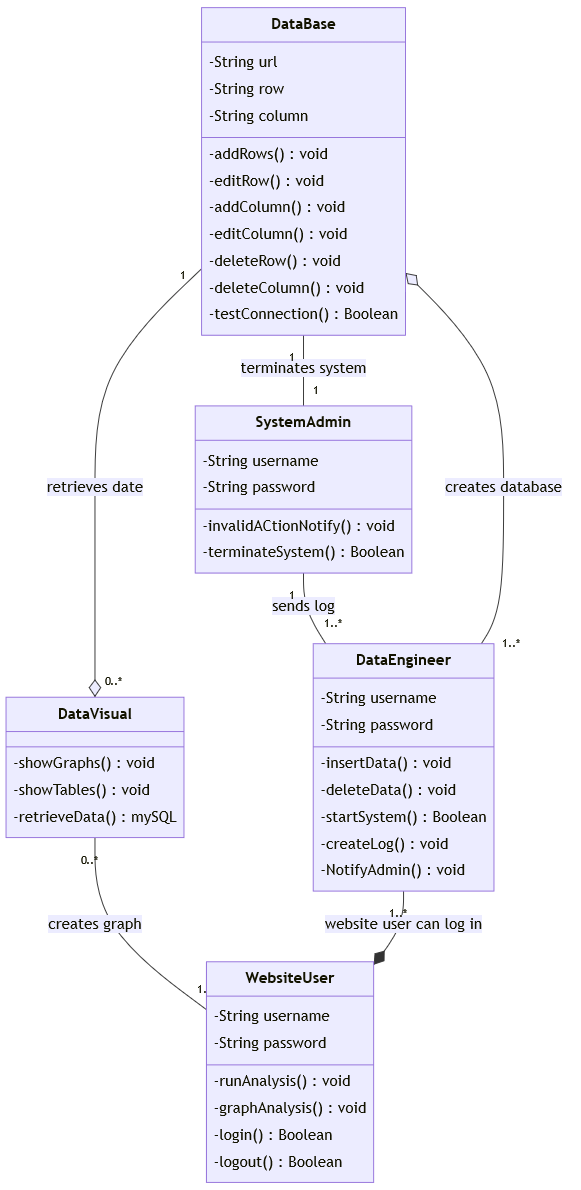
\includegraphics[height=0.6\paperheight]{./Class Diagrams/ColdCaseClassDiagram_mermaid.png}\\
			\{If this image is difficult to read, refer to the origin: \href{https://mermaid.ink/img/pako:eNqlVU1vGjEQ_SuWT21EIEBLkr2RD_WSVmrph1TtZVgPu5a8NrK9IBTx3zu2ybJ85VJO3nl-b55nPOaVF0Ygz3ihwLknCaWFOteMfk_g4QEcspwPc86ur3eL2cZ5rKeilpplzKOlBXh0zEXgAtnQ6qbfv6KPgP2WrgFFfIveSlwRXZDInvysS6kRbRBItKQx3AlE8YwVFmNuIsOcQkmga7Hrfp-_lc-YQy0cU6bcJ9-5ax132X9w7qTHXy6S3_JT2ZbV--6vjqjr9MWa8FmADhaY1LlOMrEhHTevKczYtavM-kvI5z58zNjKSHEA_YS5wlPordBBMYD1Zvb9JaHb44yhuPt8MyLqkjVWHYesWR-HCqOauj0ExUGIH2Z96geF9AScxGn_Y9Qg5ITQIoccgQo9nlNLyAUaNY4UtcbCSxPhB2MUgj5Tls6VOq0MdVBDjcfxJRHXxu4TSr0CJcX0MeT7ZrxcbM6Y2g1Uyvi-q-5da21dNnbZWjRHu_3b9eh6aut4AXQerL9gN25IU_JiyjPkVIZY2EP04KCd0fnfc9pGTzWojZPujJ04yO_gNKRSnz8lQabxpw3jPV5TU0EKemej-5z7Cskuz2gpcAGN8jnPddjaLMND-EyX3VieLUA57HFovJltdNEG0q7de91GlQGBxHrlfrMMr3opnSfNwuiFLEOchpjClfdLlw0GAe6X0lfNvF-YeuCkqKiV1ep-MpiMJncwGuPkdgyfx2NRzIf3d4vRp-FC3N4MR8C32x5fgv5rDBnwtqH8GF1_3f2jpKTbf11N_Pk?type=png)](https://mermaid.live/edit#pako:eNqlVU1vGjEQ_SuWT21EIEBLkr2RD_WSVmrph1TtZVgPu5a8NrK9IBTx3zu2ybJ85VJO3nl-b55nPOaVF0Ygz3ihwLknCaWFOteMfk_g4QEcspwPc86ur3eL2cZ5rKeilpplzKOlBXh0zEXgAtnQ6qbfv6KPgP2WrgFFfIveSlwRXZDInvysS6kRbRBItKQx3AlE8YwVFmNuIsOcQkmga7Hrfp-_lc-YQy0cU6bcJ9-5ax132X9w7qTHXy6S3_JT2ZbV--6vjqjr9MWa8FmADhaY1LlOMrEhHTevKczYtavM-kvI5z58zNjKSHEA_YS5wlPordBBMYD1Zvb9JaHb44yhuPt8MyLqkjVWHYesWR-HCqOauj0ExUGIH2Z96geF9AScxGn_Y9Qg5ITQIoccgQo9nlNLyAUaNY4UtcbCSxPhB2MUgj5Tls6VOq0MdVBDjcfxJRHXxu4TSr0CJcX0MeT7ZrxcbM6Y2g1Uyvi-q-5da21dNnbZWjRHu_3b9eh6aut4AXQerL9gN25IU_JiyjPkVIZY2EP04KCd0fnfc9pGTzWojZPujJ04yO_gNKRSnz8lQabxpw3jPV5TU0EKemej-5z7Cskuz2gpcAGN8jnPddjaLMND-EyX3VieLUA57HFovJltdNEG0q7de91GlQGBxHrlfrMMr3opnSfNwuiFLEOchpjClfdLlw0GAe6X0lfNvF-YeuCkqKiV1ep-MpiMJncwGuPkdgyfx2NRzIf3d4vRp-FC3N4MR8C32x5fgv5rDBnwtqH8GF1_3f2jpKTbf11N_Pk}{mermaid.live image}, 
			or the editing link here \href{https://mermaid.live/edit#pako:eNqlVU1vGjEQ_SuWT21EIEBLkr2RD_WSVmrph1TtZVgPu5a8NrK9IBTx3zu2ybJ85VJO3nl-b55nPOaVF0Ygz3ihwLknCaWFOteMfk_g4QEcspwPc86ur3eL2cZ5rKeilpplzKOlBXh0zEXgAtnQ6qbfv6KPgP2WrgFFfIveSlwRXZDInvysS6kRbRBItKQx3AlE8YwVFmNuIsOcQkmga7Hrfp-_lc-YQy0cU6bcJ9-5ax132X9w7qTHXy6S3_JT2ZbV--6vjqjr9MWa8FmADhaY1LlOMrEhHTevKczYtavM-kvI5z58zNjKSHEA_YS5wlPordBBMYD1Zvb9JaHb44yhuPt8MyLqkjVWHYesWR-HCqOauj0ExUGIH2Z96geF9AScxGn_Y9Qg5ITQIoccgQo9nlNLyAUaNY4UtcbCSxPhB2MUgj5Tls6VOq0MdVBDjcfxJRHXxu4TSr0CJcX0MeT7ZrxcbM6Y2g1Uyvi-q-5da21dNnbZWjRHu_3b9eh6aut4AXQerL9gN25IU_JiyjPkVIZY2EP04KCd0fnfc9pGTzWojZPujJ04yO_gNKRSnz8lQabxpw3jPV5TU0EKemej-5z7Cskuz2gpcAGN8jnPddjaLMND-EyX3VieLUA57HFovJltdNEG0q7de91GlQGBxHrlfrMMr3opnSfNwuiFLEOchpjClfdLlw0GAe6X0lfNvF-YeuCkqKiV1ep-MpiMJncwGuPkdgyfx2NRzIf3d4vRp-FC3N4MR8C32x5fgv5rDBnwtqH8GF1_3f2jpKTbf11N_Pk}{mermaid.live editor}.\}
	\caption{Class Diagram for the Cold-Cases Database system.}
	\label{fig:class_diagram}
\end{figure}
\clearpage
%-----------------------------------------------------------------------------------------
%-----------------------------------------------------------------------------------------



\section*{State Chart Diagram}

\begin{figure}[!ht]
\centering
\textbf{Author: Megan Steinmasel (Mermaid: William Jardee)}
	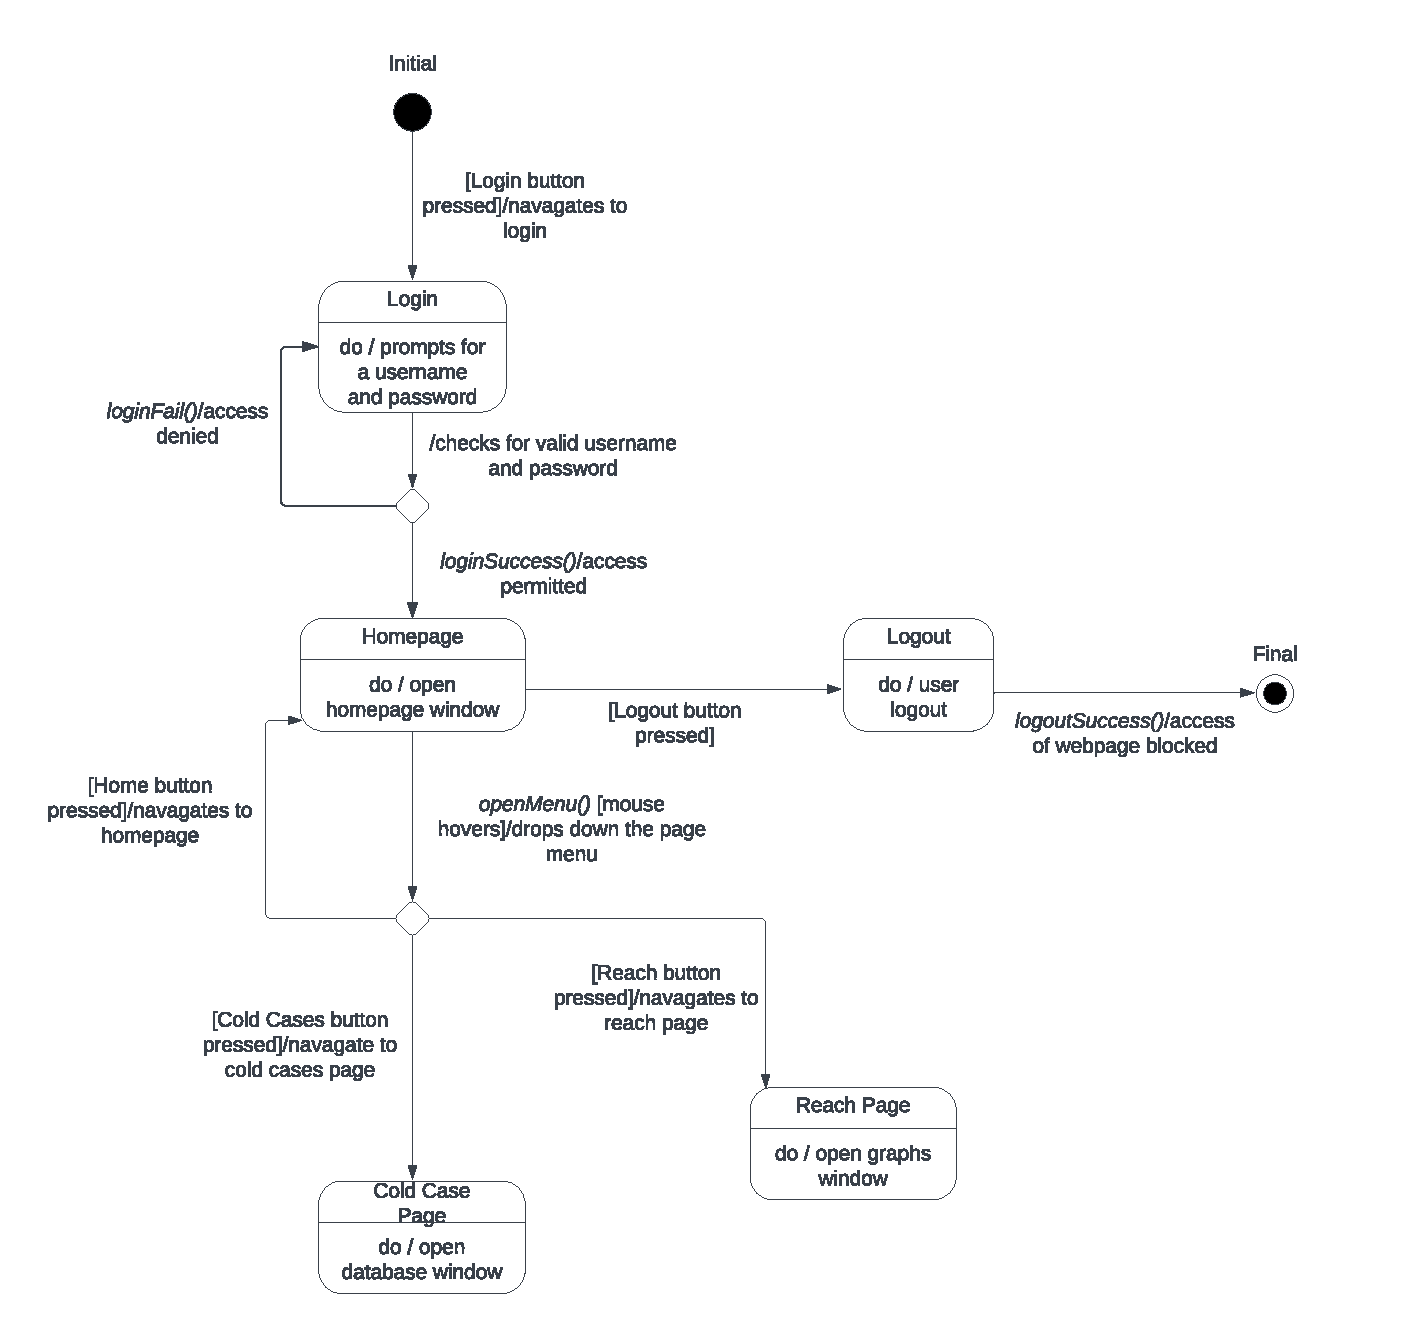
\includegraphics[width=.95\textwidth]{./State Chart/C.C. Statechart}\\
	\{If this image is difficult to read, refer to an online rendition: \href{https://mermaid.ink/img/pako:eNqlVU1vGjEQ_SuWT21EIEBLkr2RD_WSVmrph1TtZVgPu5a8NrK9IBTx3zu2ybJ85VJO3nl-b55nPOaVF0Ygz3ihwLknCaWFOteMfk_g4QEcspwPc86ur3eL2cZ5rKeilpplzKOlBXh0zEXgAtnQ6qbfv6KPgP2WrgFFfIveSlwRXZDInvysS6kRbRBItKQx3AlE8YwVFmNuIsOcQkmga7Hrfp-_lc-YQy0cU6bcJ9-5ax132X9w7qTHXy6S3_JT2ZbV--6vjqjr9MWa8FmADhaY1LlOMrEhHTevKczYtavM-kvI5z58zNjKSHEA_YS5wlPordBBMYD1Zvb9JaHb44yhuPt8MyLqkjVWHYesWR-HCqOauj0ExUGIH2Z96geF9AScxGn_Y9Qg5ITQIoccgQo9nlNLyAUaNY4UtcbCSxPhB2MUgj5Tls6VOq0MdVBDjcfxJRHXxu4TSr0CJcX0MeT7ZrxcbM6Y2g1Uyvi-q-5da21dNnbZWjRHu_3b9eh6aut4AXQerL9gN25IU_JiyjPkVIZY2EP04KCd0fnfc9pGTzWojZPujJ04yO_gNKRSnz8lQabxpw3jPV5TU0EKemej-5z7Cskuz2gpcAGN8jnPddjaLMND-EyX3VieLUA57HFovJltdNEG0q7de91GlQGBxHrlfrMMr3opnSfNwuiFLEOchpjClfdLlw0GAe6X0lfNvF-YeuCkqKiV1ep-MpiMJncwGuPkdgyfx2NRzIf3d4vRp-FC3N4MR8C32x5fgv5rDBnwtqH8GF1_3f2jpKTbf11N_Pk?type=png)](https://mermaid.live/edit#pako:eNqlVU1vGjEQ_SuWT21EIEBLkr2RD_WSVmrph1TtZVgPu5a8NrK9IBTx3zu2ybJ85VJO3nl-b55nPOaVF0Ygz3ihwLknCaWFOteMfk_g4QEcspwPc86ur3eL2cZ5rKeilpplzKOlBXh0zEXgAtnQ6qbfv6KPgP2WrgFFfIveSlwRXZDInvysS6kRbRBItKQx3AlE8YwVFmNuIsOcQkmga7Hrfp-_lc-YQy0cU6bcJ9-5ax132X9w7qTHXy6S3_JT2ZbV--6vjqjr9MWa8FmADhaY1LlOMrEhHTevKczYtavM-kvI5z58zNjKSHEA_YS5wlPordBBMYD1Zvb9JaHb44yhuPt8MyLqkjVWHYesWR-HCqOauj0ExUGIH2Z96geF9AScxGn_Y9Qg5ITQIoccgQo9nlNLyAUaNY4UtcbCSxPhB2MUgj5Tls6VOq0MdVBDjcfxJRHXxu4TSr0CJcX0MeT7ZrxcbM6Y2g1Uyvi-q-5da21dNnbZWjRHu_3b9eh6aut4AXQerL9gN25IU_JiyjPkVIZY2EP04KCd0fnfc9pGTzWojZPujJ04yO_gNKRSnz8lQabxpw3jPV5TU0EKemej-5z7Cskuz2gpcAGN8jnPddjaLMND-EyX3VieLUA57HFovJltdNEG0q7de91GlQGBxHrlfrMMr3opnSfNwuiFLEOchpjClfdLlw0GAe6X0lfNvF-YeuCkqKiV1ep-MpiMJncwGuPkdgyfx2NRzIf3d4vRp-FC3N4MR8C32x5fgv5rDBnwtqH8GF1_3f2jpKTbf11N_Pk}{mermaid.live image}, 
			or the editing link here \href{https://mermaid.live/edit#pako:eNqlVU1vGjEQ_SuWT21EIEBLkr2RD_WSVmrph1TtZVgPu5a8NrK9IBTx3zu2ybJ85VJO3nl-b55nPOaVF0Ygz3ihwLknCaWFOteMfk_g4QEcspwPc86ur3eL2cZ5rKeilpplzKOlBXh0zEXgAtnQ6qbfv6KPgP2WrgFFfIveSlwRXZDInvysS6kRbRBItKQx3AlE8YwVFmNuIsOcQkmga7Hrfp-_lc-YQy0cU6bcJ9-5ax132X9w7qTHXy6S3_JT2ZbV--6vjqjr9MWa8FmADhaY1LlOMrEhHTevKczYtavM-kvI5z58zNjKSHEA_YS5wlPordBBMYD1Zvb9JaHb44yhuPt8MyLqkjVWHYesWR-HCqOauj0ExUGIH2Z96geF9AScxGn_Y9Qg5ITQIoccgQo9nlNLyAUaNY4UtcbCSxPhB2MUgj5Tls6VOq0MdVBDjcfxJRHXxu4TSr0CJcX0MeT7ZrxcbM6Y2g1Uyvi-q-5da21dNnbZWjRHu_3b9eh6aut4AXQerL9gN25IU_JiyjPkVIZY2EP04KCd0fnfc9pGTzWojZPujJ04yO_gNKRSnz8lQabxpw3jPV5TU0EKemej-5z7Cskuz2gpcAGN8jnPddjaLMND-EyX3VieLUA57HFovJltdNEG0q7de91GlQGBxHrlfrMMr3opnSfNwuiFLEOchpjClfdLlw0GAe6X0lfNvF-YeuCkqKiV1ep-MpiMJncwGuPkdgyfx2NRzIf3d4vRp-FC3N4MR8C32x5fgv5rDBnwtqH8GF1_3f2jpKTbf11N_Pk}{mermaid.live editor}.\}
	\caption{State Chart Diagram for the Cold-Cases Database system.}
	\label{fig:state_chart_diagram}
\end{figure}
\clearpage
%-----------------------------------------------------------------------------------------
%-----------------------------------------------------------------------------------------



\section*{Activity Diagram}

\begin{figure}[!ht]
\centering
\textbf{Author: Jacob Coleman (Mermaid: William Jardee)}
	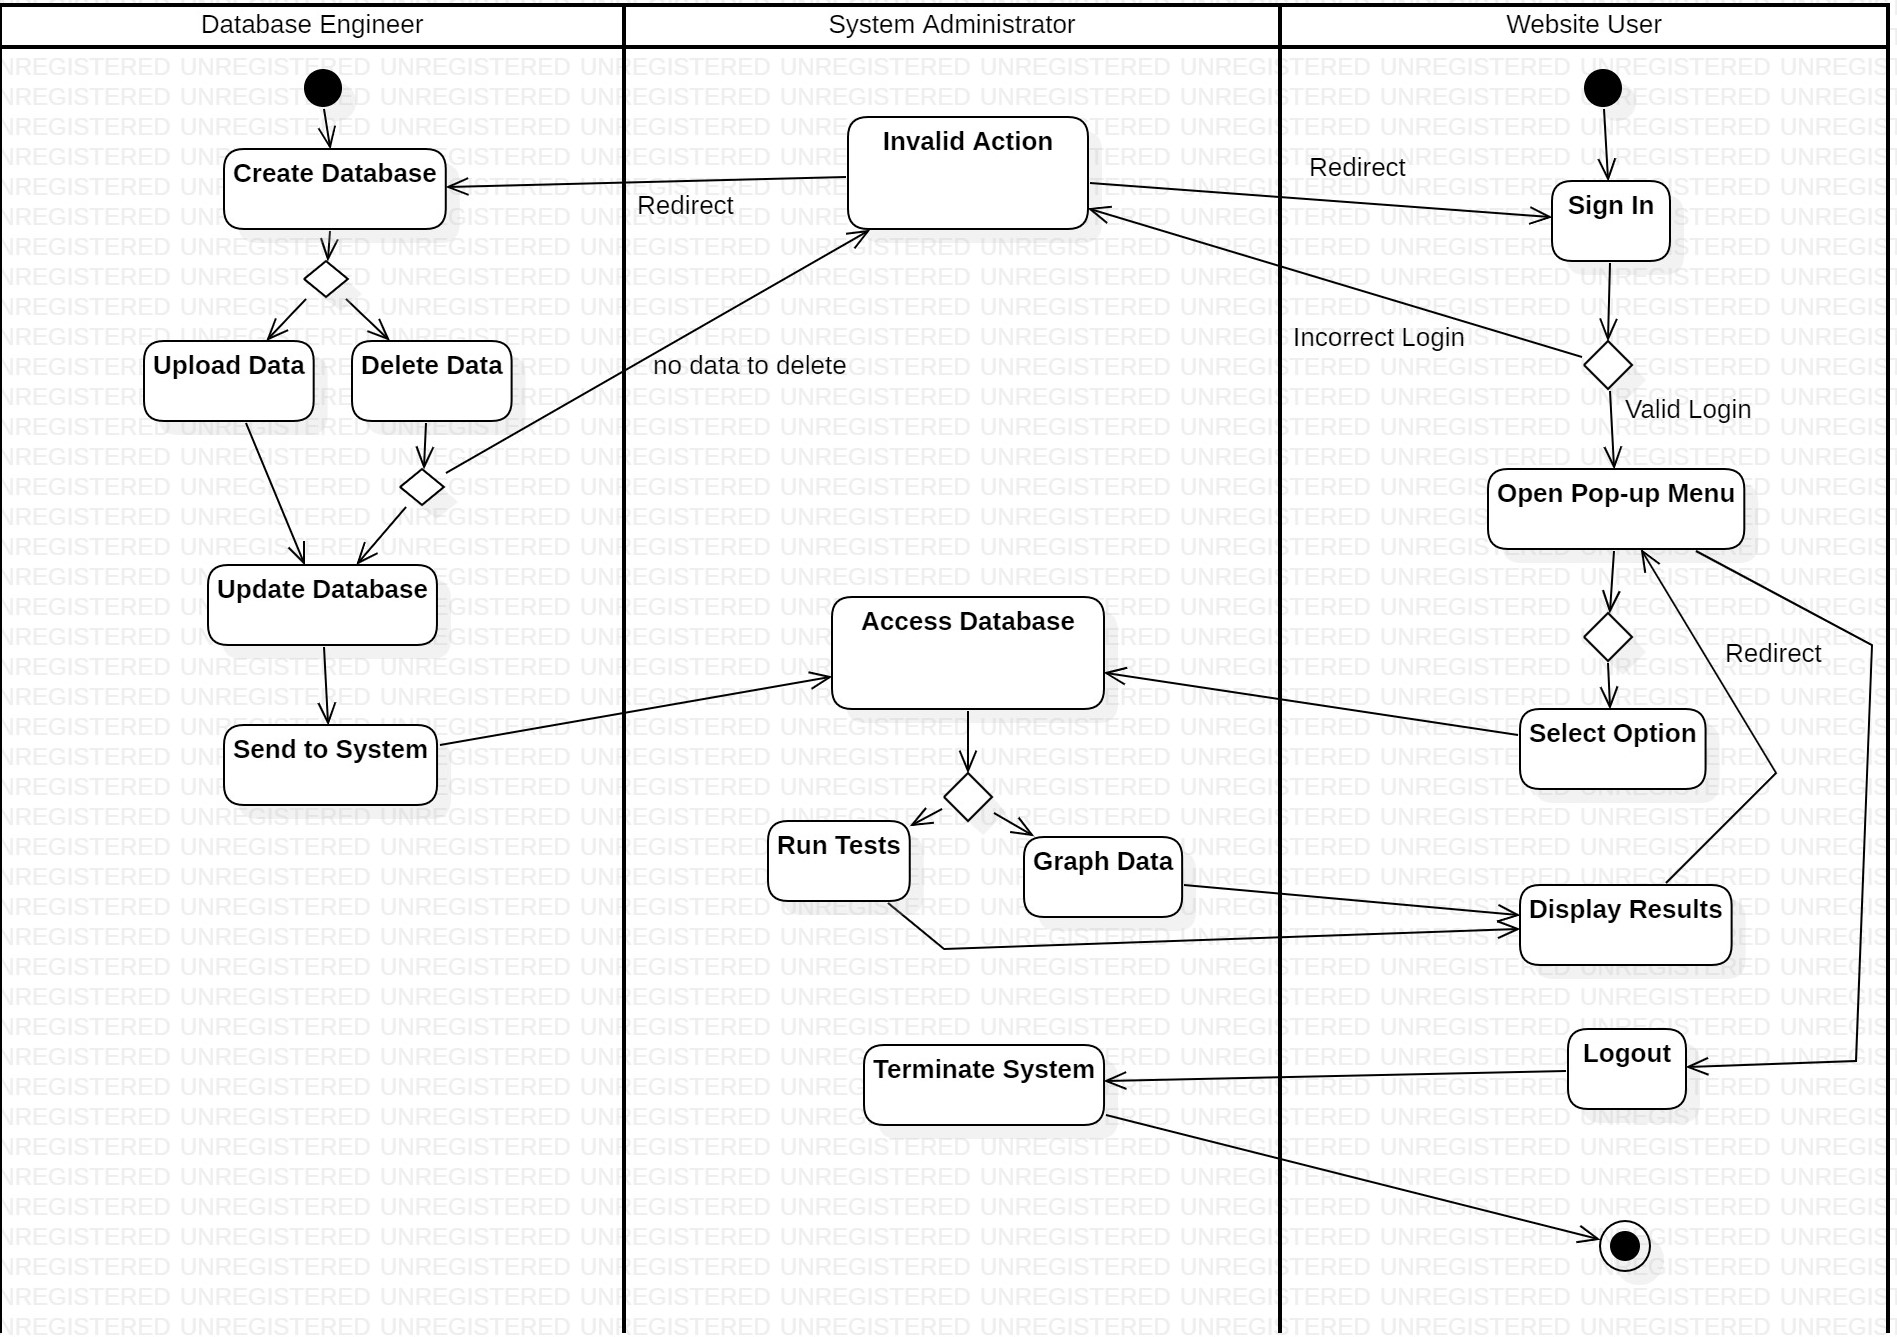
\includegraphics[width=.95\textwidth]{./Activity Diagram/activitydiagram2}\\
	\{If this image is difficult to read, refer to an online rendition: \href{https://mermaid.ink/img/pako:eNp9lW1r2zAQx7-K0cuRpLWdB8eUQlnLGGx0tCuDLSMo8sUWs2Vjyd2ykO--04Mjt0mXN5Hudzrdnf8-7wmrMyApkYoquOU0b2k1fo5WIsAfiDwNbqmiGyohuBM5FwCtZXIn1zQL0uBxJxVUwU1WccGlaqmqnctv2Kw7CS06fYON5AqCJ9mfZ-06owrR-xbw6uM1lnaNo09NWeM1mlqSQenQLZTgDg4P2WT1yew0rgRhctZ_qna5W8TFMy25ph_d6oYpXgtLKWMmOOIbxkDKV4HbtQKps3roRPAVl9Lac5fsh5Y2xSBXBS32CxNM0dstX6Qj11xgojwXmI81VSA6DHXfgAi-1M24a4ypr6wEpkxtZnHf-OQ_1XndqZXbmUdtyw2urlhRcwbX10Ome8wKYL_e4Fxg-hQvOY8rKkzVQ2r50AvFtbd7_fvx7ud4fO1U4c1OJRq5qJ7112hoH_155hTjYS-hHppSX2JbvY88eNKnLk45Hg-FqB2M6jzWW23uNWXJ4ehg-9O_PYMmZVw2Jd1p7bvVA8iu7LXm-mivRPl4a6_tU6J3vohXJ85X55FX31GetlytwGG9RpGnJQ9r-k-8Xr49sHuDjq-Rp0eTccB-9OI7DNVnx9f-pEXecJrqmcuOY8F2yr0Ww6jOpLmdEW_A_KVG3TwxErUd8iz36h0iXR8ZkQqzpDzDmW6qWxFVQAUrkuIygy1FvazIShzQtTMj8i7jOLJJuqWlhBGhnaofd4KRVLUd9E7u03D00lMZ8NCeqF2jPyA5zn4MyWqx5bm2d22J5kKpRqYXFxpPcq6KbjNhdXUheVbQVhXPy_nFPJonNIphvojpLI4ztgmXyTaahttscRlGlBwOI9JQoaP-IWmcRJNkeRnOF1E8j6MkHJEdScezSRjNZtMonMfJNEkWCzz0t64x5XByGU5ny-VsGSWzCG-ITbjvBtoiwfTgs_0Wmk_i4R9q0ioj?type=png)](https://mermaid.live/edit#pako:eNp9lW1r2zAQx7-K0cuRpLWdB8eUQlnLGGx0tCuDLSMo8sUWs2Vjyd2ykO--04Mjt0mXN5Hudzrdnf8-7wmrMyApkYoquOU0b2k1fo5WIsAfiDwNbqmiGyohuBM5FwCtZXIn1zQL0uBxJxVUwU1WccGlaqmqnctv2Kw7CS06fYON5AqCJ9mfZ-06owrR-xbw6uM1lnaNo09NWeM1mlqSQenQLZTgDg4P2WT1yew0rgRhctZ_qna5W8TFMy25ph_d6oYpXgtLKWMmOOIbxkDKV4HbtQKps3roRPAVl9Lac5fsh5Y2xSBXBS32CxNM0dstX6Qj11xgojwXmI81VSA6DHXfgAi-1M24a4ypr6wEpkxtZnHf-OQ_1XndqZXbmUdtyw2urlhRcwbX10Ome8wKYL_e4Fxg-hQvOY8rKkzVQ2r50AvFtbd7_fvx7ud4fO1U4c1OJRq5qJ7112hoH_155hTjYS-hHppSX2JbvY88eNKnLk45Hg-FqB2M6jzWW23uNWXJ4ehg-9O_PYMmZVw2Jd1p7bvVA8iu7LXm-mivRPl4a6_tU6J3vohXJ85X55FX31GetlytwGG9RpGnJQ9r-k-8Xr49sHuDjq-Rp0eTccB-9OI7DNVnx9f-pEXecJrqmcuOY8F2yr0Ww6jOpLmdEW_A_KVG3TwxErUd8iz36h0iXR8ZkQqzpDzDmW6qWxFVQAUrkuIygy1FvazIShzQtTMj8i7jOLJJuqWlhBGhnaofd4KRVLUd9E7u03D00lMZ8NCeqF2jPyA5zn4MyWqx5bm2d22J5kKpRqYXFxpPcq6KbjNhdXUheVbQVhXPy_nFPJonNIphvojpLI4ztgmXyTaahttscRlGlBwOI9JQoaP-IWmcRJNkeRnOF1E8j6MkHJEdScezSRjNZtMonMfJNEkWCzz0t64x5XByGU5ny-VsGSWzCG-ITbjvBtoiwfTgs_0Wmk_i4R9q0ioj}{mermaid.live image}, 
			or the editing link here \href{https://mermaid.live/edit#pako:eNp9lW1r2zAQx7-K0cuRpLWdB8eUQlnLGGx0tCuDLSMo8sUWs2Vjyd2ykO--04Mjt0mXN5Hudzrdnf8-7wmrMyApkYoquOU0b2k1fo5WIsAfiDwNbqmiGyohuBM5FwCtZXIn1zQL0uBxJxVUwU1WccGlaqmqnctv2Kw7CS06fYON5AqCJ9mfZ-06owrR-xbw6uM1lnaNo09NWeM1mlqSQenQLZTgDg4P2WT1yew0rgRhctZ_qna5W8TFMy25ph_d6oYpXgtLKWMmOOIbxkDKV4HbtQKps3roRPAVl9Lac5fsh5Y2xSBXBS32CxNM0dstX6Qj11xgojwXmI81VSA6DHXfgAi-1M24a4ypr6wEpkxtZnHf-OQ_1XndqZXbmUdtyw2urlhRcwbX10Ome8wKYL_e4Fxg-hQvOY8rKkzVQ2r50AvFtbd7_fvx7ud4fO1U4c1OJRq5qJ7112hoH_155hTjYS-hHppSX2JbvY88eNKnLk45Hg-FqB2M6jzWW23uNWXJ4ehg-9O_PYMmZVw2Jd1p7bvVA8iu7LXm-mivRPl4a6_tU6J3vohXJ85X55FX31GetlytwGG9RpGnJQ9r-k-8Xr49sHuDjq-Rp0eTccB-9OI7DNVnx9f-pEXecJrqmcuOY8F2yr0Ww6jOpLmdEW_A_KVG3TwxErUd8iz36h0iXR8ZkQqzpDzDmW6qWxFVQAUrkuIygy1FvazIShzQtTMj8i7jOLJJuqWlhBGhnaofd4KRVLUd9E7u03D00lMZ8NCeqF2jPyA5zn4MyWqx5bm2d22J5kKpRqYXFxpPcq6KbjNhdXUheVbQVhXPy_nFPJonNIphvojpLI4ztgmXyTaahttscRlGlBwOI9JQoaP-IWmcRJNkeRnOF1E8j6MkHJEdScezSRjNZtMonMfJNEkWCzz0t64x5XByGU5ny-VsGSWzCG-ITbjvBtoiwfTgs_0Wmk_i4R9q0ioj}{mermaid.live editor}.
			Notice that the Mermaid version has numerous formatting issues. Mermaid does not support Activity Diagrams yet.\}
	\caption{Activity Diagram for the Cold-Cases Database system.}
	\label{fig:activity_diagram}
\end{figure}

\end{document}
